% ------------------------------------------------------------------------------
% Este fichero es parte de la plantilla LaTeX para la realización de Proyectos
% Final de Grado, protegido bajo los términos de la licencia GFDL.
% Para más información, la licencia completa viene incluida en el
% fichero fdl-1.3.tex

% Copyright (C) 2012 SPI-FM. Universidad de Cádiz
% ------------------------------------------------------------------------------


En esta sección se describen todos los aspectos relativos a la planificación del
proyecto: metodología, organización, costes, planificación y gestión de riesgos.

\section{Metodología de desarrollo}

Como metodología de desarrollo para la elaboración del proyecto, nos hemos
basado en el modelo de ciclo de vida de desarrollo en espiral. Este modelo de
desarrollo se centra en dividir el proyecto en segmentos más pequeños y
proporcionar más facilidad de cambio en el proceso de desarrollo. En este
modelo, se combinan las principales características del desarrollo
iterativo, con las del desarrollo en cascada, de forma que en cada uno de las
iteraciones en la espiral, recoge todas fases del modelo en cascada, de
tal forma, que al final de cada iteración, obtenemos una porción de software,
y en las sucesivas iteraciones se obtienen versiones incrementales de la misma
pieza software. Tal y como explicamos en el capítulo anterior, nuestro proyecto
lo hemos dividido en varias piezas software ``independientes'', de tal forma
haciendo uso de este modelo, nos permitirá realizar el desarrollo por partes,
obteniendo en cada una de las iteraciones de la espiral, una de las piezas
software definidas anteriormente.

Para el modelo de ciclo de vida de desarrollo en espiral, se definen cuatro
fases, las cuales son las que se repiten en cada una de las iteraciones de la
espiral. Estas fases son las siguientes:
\begin{itemize}
    \item \textbf{Definición de objetivos:} Exceptuando la planificación inicial,
           que es llevada a cabo al comienzo del proyecto, en esta fase en cada
           una de las iteraciones de la espiral se especifican y analizan los
           requisitos que deberá cumplir el componente software, al final de la
           iteración para cumplir cada uno de los objetivos en los que hemos
           dividido el proyecto.
    \item \textbf{Análisis de riesgos:} En esta fase se evalúan los posibles
           riesgos y eventos no deseados que puedan surgir durante la ejecución
           de la iteración, para que en la fase de desarrollo y pruebas, se
           puedan evaluar los mismos y buscar las alternativas posibles para
           solventarlos.
    \item \textbf{Desarrollo y pruebas:} En este apartado se realizan las
           tareas propias que su nombre indica, se lleva a cabo el diseño e
           implementación de los requisitos especificados, y se prueban los
           mismos. Además, en este apartado, como se acaba de comentar, se
           evalúan las posibles alternativas para solventar los posibles riesgos
           existentes. Al final de esta fase, se obtiene la nueva versión
           incremental del software.
    \item \textbf{Planificación:} En esta fase se revisan el producto obtenido,
           y se decide si se continúa con la siguiente iteración.
\end{itemize}


\section{Planificación del proyecto}
A continuación se va a realizar una estimación temporal del tiempo que se
empleará en la elaboración del proyecto. Para ello, vamos a dividir el proyecto
en una serie de fases, las cuales según la complejidad y extensión de las
mismas, se le asignará un tiempo estimado para su finalización.

\subsection{Especificación de las Fases}

Las fases en las que vamos a dividir nuestro proyecto para realizar la
estimación temporal, son las siguientes:

\begin{itemize}
    \item \textbf{Estudio inicial:} este apartado hace referencia al estudio
           de la propuesta de proyecto, redacción del proyecto y motivaciones
           del mismo. Comprende desde las primeras reuniones con los tutores del
           proyecto donde se propone el mismo, hasta el momento de la asignación
           de este.
    \item \textbf{Preparación del entorno:} esta parte se refiere a todas las
           tareas realizadas para la preparación del entorno de trabajo para
           elaborar el proyecto. Desde la solicitud de apertura de un espacio de
           trabajo y un repositorio SVN para alojar el proyecto, hasta la
           selección e instalación de las herramientas necesarias para realizar
           el mismo, como pueden ser el IDE, el sistema de control de versiones,
           servidores o configuración de la máquina.
    \item \textbf{Fase de Análisis\footnote{\label{pie}Estos apartados se
           repetirán varias veces a lo largo del desarrollo del proyecto, ya que
           al hacer uso de una metodología de desarrollo en espiral, en cada una
           de las iteraciones de la metodología, tendremos que volver a revisar
           cada uno de los requisitos, para determinar si se cumplen o si estos
           se adaptan a los requisitos verdaderos de la aplicación, y continuar
           con la implementación y/o corrección de los requisitos existentes y
           realizar las pruebas de los mismos.}:} el apartado de fase de
           análisis, se corresponde totalmente con la fase de análisis del ciclo
           de vida del software. Aquí se especifican los requisitos funcionales
           y no funcionales que debe de poseer la aplicación, los distintos
           actores que pueden intervenir en él, se detallan los casos de uso y
           se hace una especificación de los datos que manejará nuestra
           aplicación.
    \item \textbf{Fase de Diseño$^{\ref{pie}}$:} dentro del ciclo de vida del
           software, esta fase es la que aparece justo a continuación de la fase
           de análisis. Es esta fase se baja un nivel de abstracción más,
           respecto de la fase anterior. Aquí se detallará a nivel de
           operaciones, como se llevarán a cabo las distintas funciones que debe
           cumplir nuestro software. Además, se proporcionará un diagrama de
           persistencia de los datos que maneja nuestra aplicación en una base
           de datos.
    \item \textbf{Implementación$^{\ref{pie}}$: } esta fase hace referencia a
           el apartado más técnico del desarrollo del producto. En esta fase se
           pasa de la especificación en papel, a la codificación del mismo en el
           lenguaje de programación seleccionado. Esta fase es de las más
           extensas y a su vez de las más importantes, ya que es donde se
           obtendrá el producto software final.
    \item \textbf{Pruebas$^{\ref{pie}}$: } esta fase, no menos importante que
           la de implementación, se llevará a cabo a la vez que la
           implementación. La fase de pruebas, será la responsable del control
           de calidad, de tal forma que en ella se descubran los posibles
           errores tanto de codificación como de funcionamiento de la aplicación.
           En esta fase se asegurará que el software contenga unos mínimos de
           calidad, seguridad y fiabilidad.
    \item \textbf{Documentación: } Este apartado abarca todo el ciclo de vida
           del desarrollo del proyecto, y en él se detallarán todas y cada una
           de estas fases. Esta fase abarcará desde el momento inicial del
           proyecto, hasta el final del mismo. Este apartado además de los
           detalles técnicos de la aplicación, incluirá los manuales de usuario,
           las instrucciones de instalación y despliegue, las estimaciones de
           tiempo y conclusiones.
\end{itemize}

\subsection{Diagrama de Gantt Inicial}

En el diagrama de Gantt de la Figura \ref{fig:GanttInicial}, se pueden
apreciar cada una de las fases comentadas anteriormente, expresadas en función
del tiempo que se estima que se empleará en cada una de ellas:

\subsection{Diagrama de Gantt con los tiempos reales}

A continuación también se muestra el diagrama de gantt (Figuras
\ref{fig:GanttFinal1} y \ref{fig:GanttFinal2}), el cual se ha obtenido una vez
finalizado el proyecto, con los tiempos reales utilizados, de forma que se pueda
realizar una comparación, con los tiempos que se estimaron en un principio.

Tal y como se puede apreciar en las figuras, los tiempos estimados de duración
del proyecto se han ajustado bastante bien a los tiempos que finalmente se han
necesitado para la ejecución del proyecto. Inicialmente se estimó una duración
total de 12 meses, desde octubre de 2012 hasta octubre de 2013, habiéndose
excedido el proyecto únicamente en un mes (finalizado en noviembre de 2013).

\newpage

\begin{figure}[H]
    \begin{center}
        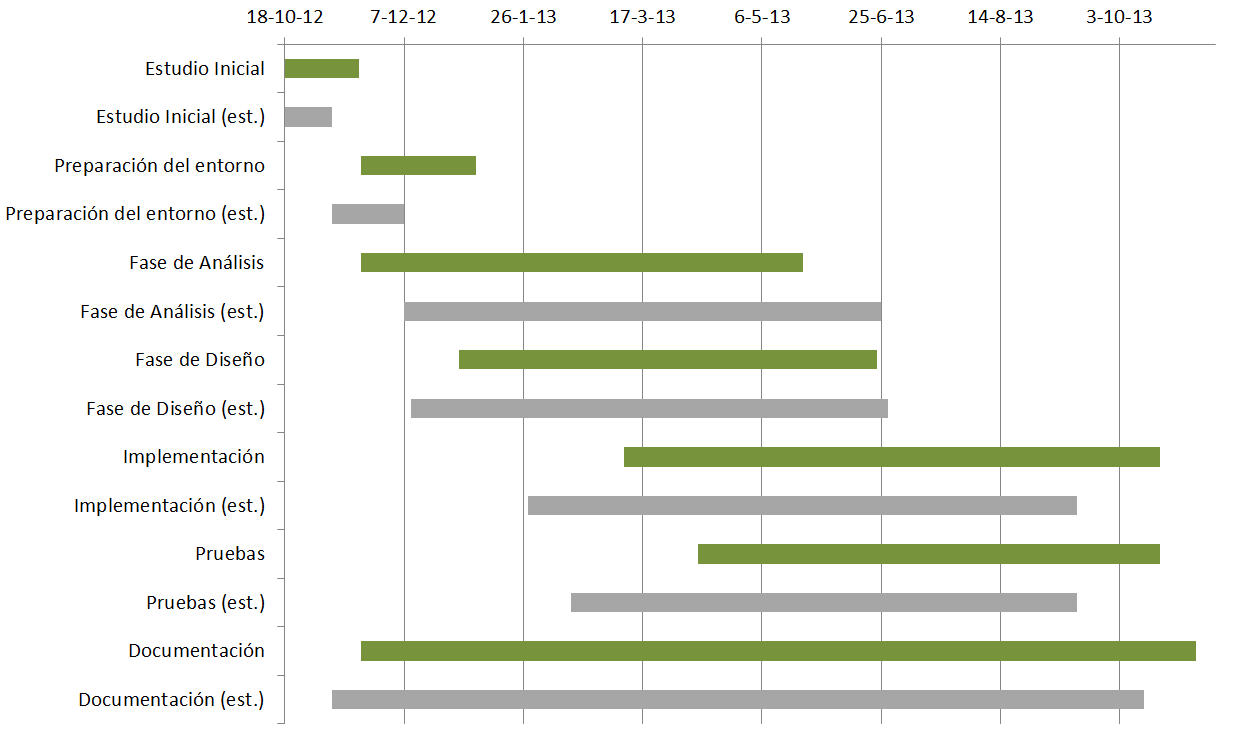
\includegraphics[width=0.7\textwidth]{diagrama_gantt.png}
    \end{center}
    \caption{Diagrama de Gantt con estimación temporal}
    \label{fig:GanttInicial}
\end{figure}

\begin{figure}[H]
    \begin{center}
        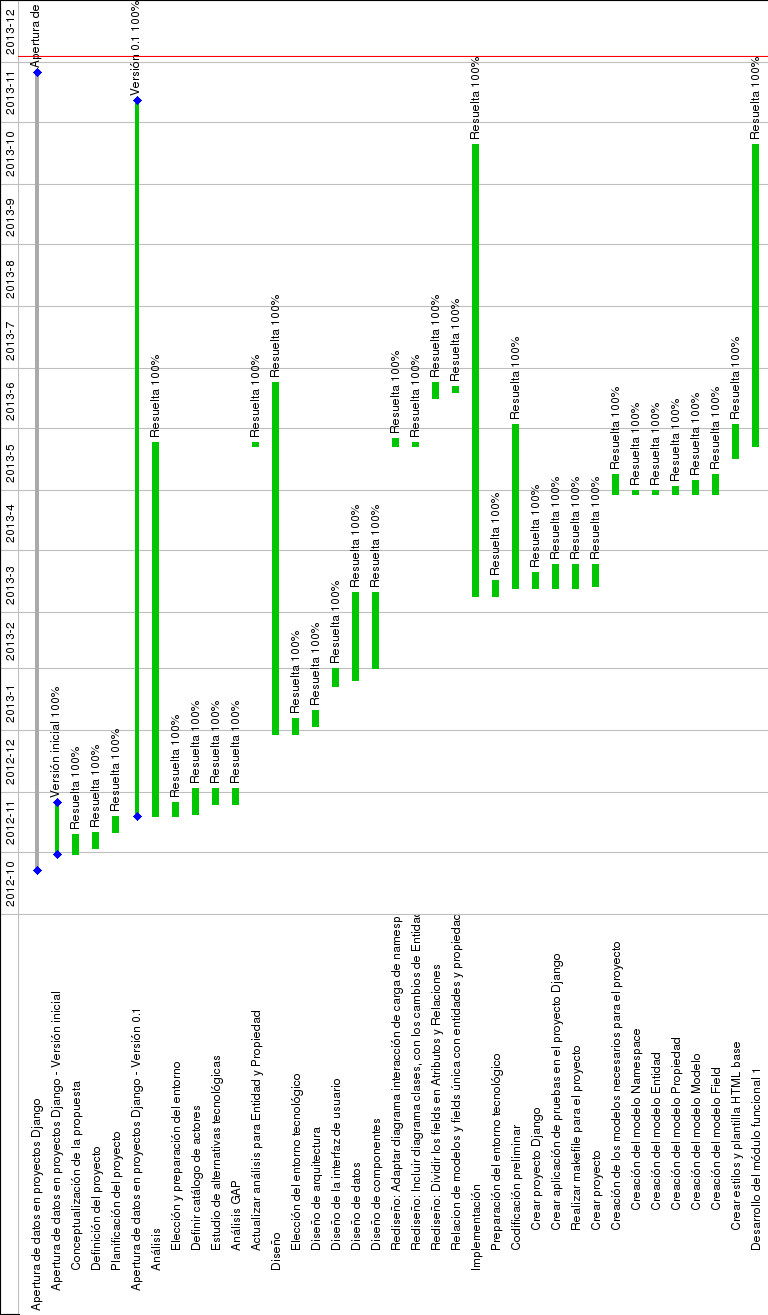
\includegraphics[width=0.85\textwidth]{gantt1.png}
    \end{center}
    \caption{Diagrama de Gantt con los tiempos finales (Parte 1)}
    \label{fig:GanttFinal1}
\end{figure}

\begin{figure}[H]
    \begin{center}
        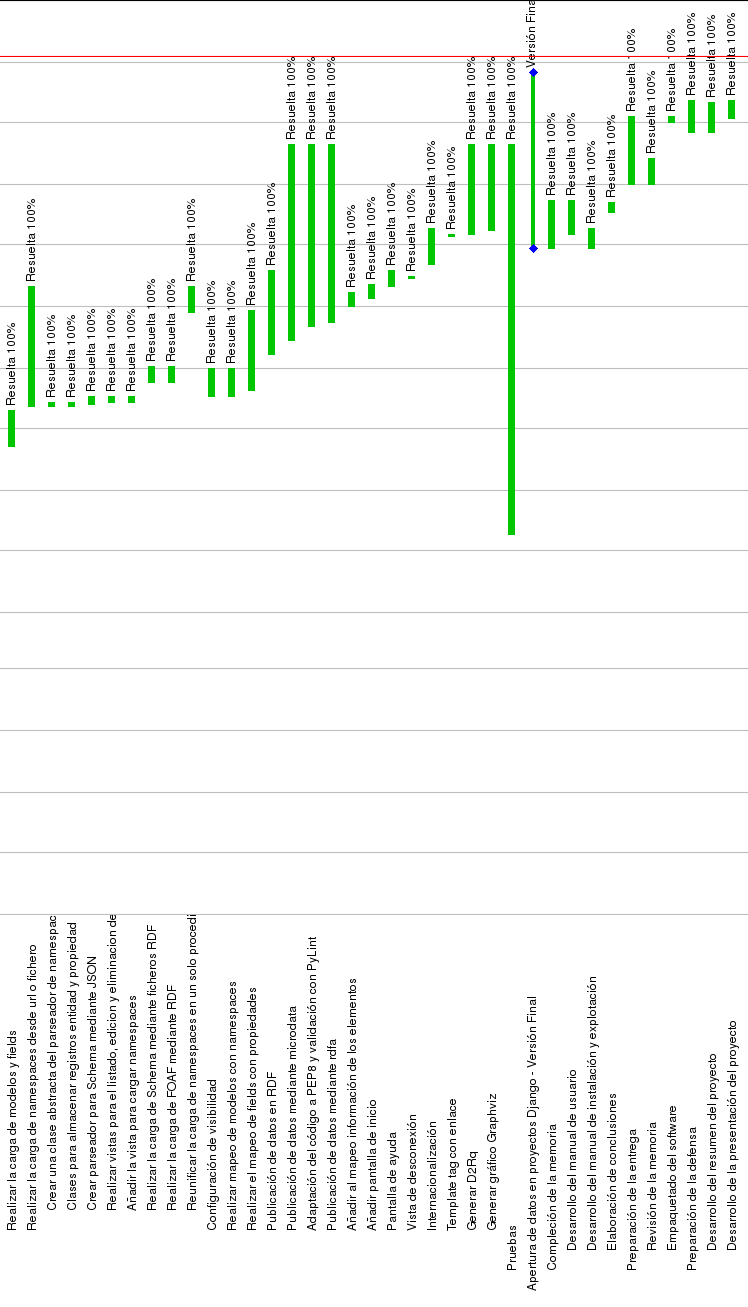
\includegraphics[width=0.85\textwidth]{gantt2.png}
    \end{center}
    \caption{Diagrama de Gantt con los tiempos finales (Parte 2)}
    \label{fig:GanttFinal2}
\end{figure}

\section{Organización}

\section{Roles existentes}

El conjunto de personas que componen a la organización involucrada en el
desarrollo del proyecto, son las siguientes:
\begin{itemize}
    \item \textbf{Desarrollador:} El desarrollador del proyecto, es el alumno
           que está llevando a cabo dicho proyecto informático. Desempeña los
           papeles de analista informático, de desarrollador informático e
           ingeniero de test. Sus funciones son las de analizar y diseñar el
           software, así como de desarrollar el mismo cumpliendo las
           especificaciones, realizar los tests de calidad oportunos y
           documentar todo el proceso de desarrollo.
    \item \textbf{Tutores:} Los tutores del proyectos, tienen como cometido
           guiar al alumno en el desarrollo del mismo. Se puede decir que
           realizan un papel similar al cliente que contrata la realización del
           software, se encargan de proponer el desarrollo del proyecto y de
           proponer los objetivos que debe cumplir el mismo. Además, también
           ayudan al alumno en el proceso de desarrollo, aportando ideas y
           posibles soluciones.
\end{itemize}

Durante el desarrollo del proyecto, el alumno como se acaba de indicar, será el
indicado de realizar todo el proceso del ciclo de vida del software.
Puntualmente, mantendrá reuniones con los tutores del proyecto, de forma que
estos puedan tener una visión del avance del proyecto a lo largo del tiempo. Los
tutores del proyecto, en cada una de estas reuniones, podrán aportar posibles
ideas, o nuevos objetivos que deba cumplir el software, guiando al alumno en la
consecución del mismo.

\section{Recursos inventariables}

En todo proyecto informático, además del factor humano, entran en escena otra
serie de factores, como son los tecnológicos, los cuales servirán al alumno en
la consecución de sus objetivos. En la Tabla \ref{tab:inventario}, se muestra
un inventario de las herramientas, tanto hardware como software, utilizadas
para la elaboración del proyecto:

\begin{center}
    \tablefirsthead{%
        \hline
        \multicolumn{1}{|c|}{\textbf{Recurso inventariable}} &
        \multicolumn{2}{c|}{\textbf{Descripción}} \\
        \hline
    }
    \tablehead{%
        \hline
        \multicolumn{3}{|l|}{\small\sl continuación de la página anterior}\\
        \hline
        \multicolumn{1}{|c|}{\textbf{Elemento inventariable}\hspace{5.5mm}} &
        \multicolumn{2}{c|}{\textbf{Descripción}} \\
        \hline
    }
    \tabletail{%
        \hline
        \multicolumn{3}{|r|}{\small\sl continua en la siguiente página}\\
        \hline
    }
    \tablelasttail{\hline}
    \bottomcaption{Tabla con inventario de materiales}
    \label{tab:inventario}
    \begin{supertabular}{|l@{\hspace{6.5mm}}|l@{\hspace{5.5mm}}|l@{\hspace{5.5mm}}|}
        \multirow{5}{3.5cm}{Hardware} & Procesador & AMD Athlon II x3 460\\
        & Memoria RAM & 8GB DDR3\\
        & Tarjeta Gráfica & NVIDIA GeForce GTX 550 Ti\\
        & Disco Duro & Seagate 1TB SATA3 7200rpm\\
        & Grabadora DVD & LG GH24NS90 DVD 24X\\
        & Monitor & Samsung SyncMaster 2243LNX\\
        \hline
        Sistema operativo & \multicolumn{2}{l|}{Linux Mint 14 Nadia}\\
        \hline
        Editor de textos & \multicolumn{2}{l|}{Gedit 3.4.1}\\
        \hline
        Python & \multicolumn{2}{l|}{Versión 2.7}\\
        \hline
        Django & \multicolumn{2}{l|}{Versión 1.4.0}\\
        \hline
        iPython & \multicolumn{2}{l|}{Interprete interactivo de Python}\\
        \hline
        Dia & \multicolumn{2}{l|}{Software para la generación de gráficos.}\\
        \hline
        Gimp & \multicolumn{2}{l|}{Software para la edición de imágenes.}\\
        \hline
        ConceptDraw Office & \multicolumn{2}{l|}{Software para la generación de diagramas.}\\
        \hline
        Apache & \multicolumn{2}{l|}{Servidor web.}\\
    \end{supertabular}
\end{center}

Para los recursos de tipo software, se ha intentado usar en todo momento
software de tipo libre, de tal forma que se reduzcan los costes al máximo.


\section{Costes}

Para llevar a cabo una estimación de los costes de producción, a parte de tener
una estimación del tiempo y recursos necesarios para llevar a cabo el proyecto,
también es necesario conocer el precio unitario de cada uno de estos recursos.
Si bien, los recursos materiales es de un coste conocido, ya que conocemos de
cuales de ellos necesitamos disponer, y el coste de los mismos. Respecto a
materiales como puede ser el ordenador personal, mobiliario, y demás elementos
de los que debe de poseer cualquier empresa, no deben de tenerse en cuenta su
coste total, ya que estos no son específicos para un puesto en concreto, sino
que se mantendrán en la empresa y su precio se amortizará a lo largo del tiempo.
Normalmente el tiempo de amortización de los mismos, se estima en tres años, por
lo que al haber estimado una duración de un año para el proyecto, contemplaremos
solo un 33\% del precio de los mismos. De esta forma, si suponemos que
conociendo que el coste del equipo informático es de 500\euro, nos quedará un
coste total de 165\euro.

Para estimar el costo de los recursos humanos que intervendrán en el desarrollo
del proryecto software, deberemos de tener en cuenta tanto el número de personas
implicadas, como la duración del proyecto, como el sueldo que habría que
abonarle a cada uno de los participantes en el proyecto. Este proyecto, al
tratarse de un proyecto de pequeña envergadura, será realizado únicamente por
una persona, que trabajará durante 12 meses, que son los que se han estimado
para la duración del proyecto.

En la siguiente Tabla (\ref{tab:costorecursos}) se reflejan los distintos
recursos necesarios para elaborar el proyecto, con los costos y unidades
necesarias asociados de los mismos:

\begin{table}[H]
    \begin{center}
        \begin{tabular}{||c|p{7.5cm}|c||}
            \hline
            \hline
            \textbf{Recurso} & \textbf{Descripción} & \textbf{Coste} \\
            \hline
            \hline
            Ingeniero Informático & Es el encargado de realizar tanto la
            documentación del proyecto, como la implementación del mismo.
            & 1 persona/mes \\
            \hline
            Ordenador Personal & Es el equipo que utilizará el ingeniero
            informático en su puesto de trabajo. & 165\euro \\
            \hline
            Local y mobiliario & Son los gastos del local y derivados del mismo
            (luz, agua, mesa, etc\ldots) donde se va a realizar el proyecto.
            & 30\euro/mes \\
            \hline
            Material de oficina & Hace referencia a papel, bolígrafos,
            etc\ldots & 50\euro \\
            \hline
            \hline
        \end{tabular}
    \end{center}
    \caption{Tabla de costos de los recursos}
    \label{tab:costorecursos}
\end{table}

Una vez conocemos todos los recursos implicados en la elaboración del proyecto,
es necesario tener una estimación del sueldo promedio de un programador
informático en España. Infojobs posee una herramienta \cite{salarioinfo}, la
cual nos permite consultar el sueldo promedio según el puesto de trabajo que
desempeñe el trabajador. Tal y como se puede observar, el salario medio de un
ingeniero informático en España, ronda la cuantía de los \EUR{17567} anuales.
Aunque, para la realización de este proyecto, no se va a tener una dedicación
total, sino que se tratará de una dedicación parcial (aproximadamente una cuarta
parte de lo que dedicaría un trabajador normal), por lo que del total de horas
mensuales que un trabajador normal dispone (alrededor de unas 152 horas),
estimamos que se emplearán aproximadamente unas 38 horas mensuales, de tal forma
que calculando la proporción, nos queda un coste total de \EUR{366} por mes,
para la dedicación que va a tener el ingeniero al proyecto. Finalmente podemos
decir que, si el proyecto tiene un tiempo estimado de 12 meses, y el trabajador
percibirá una cantidad de \EUR{366} cada uno de los meses, el coste total del
trabajador será de \EUR{4.392}.

De esta forma, una vez que conocemos tanto la cantidad como el costo de todos
los recursos implicados en la elaboración del proyecto (tanto humanos como
materiales) y conocemos también la estimación temporal que hicimos
anteriormente, podemos estimar un costo total para el proyecto, el cual se
refleja en la Tabla \ref{tab:costetotal}:

\begin{table}[H]
    \begin{center}
        \begin{tabular}{||c|c|c|c||}
            \hline
            \hline
            \textbf{Unidades} & \textbf{Recurso} & \textbf{Coste unitario} & \textbf{Coste total} \\
            \hline
            \hline
            12 & Ingeniero informático & 366\euro & 4.392\euro \\
            \hline
            1 & Ordenador personal & 165\euro & 165\euro \\
            \hline
            12 & Local & 30\euro & 360\euro \\
            \hline
            1 & Material de oficina & 50\euro & 50\euro \\
            \hline
            \multicolumn{3}{||r|}{\textbf{Total}} & \textbf{4.967\euro} \\
            \hline
            \hline
        \end{tabular}
    \end{center}
    \caption{Tabla de coste total}
    \label{tab:costetotal}
\end{table}

Los costes finales se han calculado en función de 12 meses, ya que en la
planificación que se ha hecho anteriormente y que podemos apreciar en el
diagrama de Gantt (Figura \ref{fig:GanttInicial}), el coste temporal total
comprendía desde Octubre de 2012 hasta Septiembre de 2013, lo que hace un total
de 12 meses.

\section{Gestión de riesgos}

Dentro de todo proyecto, pueden darse a lugar una serie de riesgos, los cuales
complicarían o retrasaría los plazos fijados en la planificación del mismo.
Dentro de estos riesgos, pueden entrar en juego distintos factores, ya sean
humanos o de cualquier otro tipo de índole. En este apartado, vamos a hacer una
descripción de los posibles riesgos que podrían tener lugar, los cuales
comprometiesen el cumplimiento de la planificación. Para la descripción de estos
posibles riesgos, nos vamos a basar en los descritos en el MAGERIT V3
\cite{mageritv3} para determinar los riesgos de tipo genérico que se puedan dar,
y además citaremos otra serie de riesgos específicos del proyecto, los cuales
también retrasarían los plazos estimados en la planificación. Todos estos
riesgos deben de estar descritos dentro de la política de protección de datos de
cualquier empresa.
\begin{itemize}
    \item \textbf{Riesgos de tipo genéricos.}
    \begin{itemize}
        \item \textbf{Errores del administrador (E.2):} equivocaciones de personas
               con responsabilidades de instalación y operación.
        \item \textbf{Destrucción de información (E.18):} perdida de la
               información almacenada del proyecto.
        \item \textbf{Pérdida de equipos (E.25):} la pérdida de equipos provoca
               directamente la carencia de un medio para prestar los servicios,
               es decir una indisponibilidad. 
        \item \textbf{Indisponibilidad del personal (E.28):} ausencia accidental
               del puesto de trabajo: enfermedad, alteraciones del orden público,
               etc\ldots
        \item \textbf{Daños por agua (I.2):} escapes, fugas, inundaciones:
               posibilidad de que el agua acabe con los recursos del sistema.
        \item \textbf{Contaminación mecánica (I.3):} vibraciones, polvo, suciedad,
               \ldots
        \item \textbf{Avería de origen físico o lógico (I.5):} fallos en los
               equipos y/o fallos en los programas. Puede ser debida a un defecto de
               origen o sobrevenida durante el funcionamiento del sistema.
        \item \textbf{Corte del suministro eléctrico (I.6):} cese de la
               alimentación de potencia.
    \end{itemize}
    \item \textbf{Riesgos de tipo específicos del proyecto.}
    \begin{itemize}
        \item \textbf{Cambios en la especificación de los vocabularios:} si se
            introdujesen cambios a la hora de la especificación de los
            vocabularios, haciendo uso de una nomenclatura diferente, habría que
            modificar el parseador de ficheros XML que se encargue de dicha
            función, añadiendo la nueva nomenclatura.
        \item \textbf{Cambios en la estructura de la base de datos:} si por la
            aparición de nuevas necesidades o por deficiencias en la estuctura
            actual se debiesen hacer cambios en la base de datos, se debería de
            volver nuevamente al apartado de diseño, para definir la nueva
            estructura de la misma, determinar los sistemas donde afectarán
            dichos cambios y si fuese necesario, definir herramientas de
            migración de los datos a las nuevas estructuras, para evitar la
            pérdida de datos.
        \item \textbf{Modificación de funcionalidades existentes:} si alguna de
            las funcionalidades especificadas en el proyecto se modificasen, se
            debería de volver al apartado de análisis y diseño, para modificar
            los diagramas de caso de uso e interacción de dicha funcionalidad,
            para posteriormente pasar a la modificación de la funcionalidad.
    \end{itemize}
\end{itemize}

Para la subsanación de los riesgos que provocan una pérdida de datos, o un
deterioro de los mismos, como son los riesgos marcados con los códigos E.2,
E.18, E.25, I.2, I.3, I.5 e I.6, se hará uso de un sistema de control de 
versiones (en
nuestro caso se hace uso del sistema subversion), el cual permita en todo
momento mantener una copia de cada una de las versiones que existen del proyecto,
garantizando la disponibilidad e integridad de los datos. Asímismo, este
sistema de control de versiones, se encontrará en otra máquina ajena a la
máquina donde se está desarrollando el proyecto, y en un edificio distinto. De
esta forma, evitamos posibles pérdidas de información por causas naturales,
subidas de tensión, o deterioro de componentes físicos de la máquina donde se
está realizando el proyecto.

En el ámbito de los riesgos provocados por causas humanas, debidas a la
indisponibilidad del persona, al tratarse de un equipo de desarrollo bastante
reducido, compuesto únicamente por una persona, las precauciones que se han
tomando, han sido las de contemplar las posibles bajas por enfermedad o
indisponibilidad por parte del personal, dentro de los plazos estipulados de
realización del proyecto, intentando ajustar los plazos siempre todo lo posible,
pero dando siempre cierto margen en los tiempos (teniendo siempre en cuenta que
los costes y tiempos se encuentren siempre dentro de límites razonables), de tal
forma que un posible contratiempo de este tipo, no altere de sobremanera los
tiempos de entrega, prologándolos demasiado en el tiempo.

